\section{Design Phase} \label{designPhase}

\subsection{Third Party Libraries}

\paragraph{Cinder \cite{developers_davis}} \textit{Cinder} is a free, open-source graphics engine for \CPP. It provides a simple way to access OpenGL, ImGui and other tools, such as image loading and saving, optimised rendering in 2D and 3D, and more. I am using \textit{Cinder} for this project instead of doing all the graphics processing with raw OpenGL because it dramatically simplifies the code and reduces the scope for hard-to-fix bugs.

This project uses a modified version of \textit{Cinder} with updated libraries and a few extra features. Most significantly, this modified version includes a much newer version of ImGui and an altered build configuration to fix common compile errors on some platforms.

\paragraph{LibRapid \cite{Davis_LibRapid_Optimised_Mathematics_2023}} \textit{LibRapid} is a high-performance library for mathematical applications, including optimised vector classes, complex number types and general mathematical functions. However, this library's most helpful feature is its support for MPIR and MPFR, which are highly-optimised multi-precision implementations. This will allow floating point calculations with more than 64 bits.

Incorporating an efficient multi-precision implementation into the project could allow for ``infinite'' fractal zooms since traditional floating-point limitations would no longer constrain the software.

Another feature of \textit{LibRapid} used heavily in this project is the compiler- and system-agnostic macro definitions. Useful features like inlining of functions, no-discard specifiers and more are not implemented by all compilers and sometimes work differently on different operating systems. LibRapid implements macros which automatically detect the relevant information and define the most suitable replacement. This isn't strictly required for the project, but it might result in a slight performance improvement and can help reduce bugs.

\paragraph{Cinderbox} Both of the afore mentioned libraries are packaged with \textit{Cinderbox} for simple integration into \textit{CMake} projects.

\subsection{Library Heirarchy}

\FloatBarrier
\begin{figure*}[htp]
    \centering
    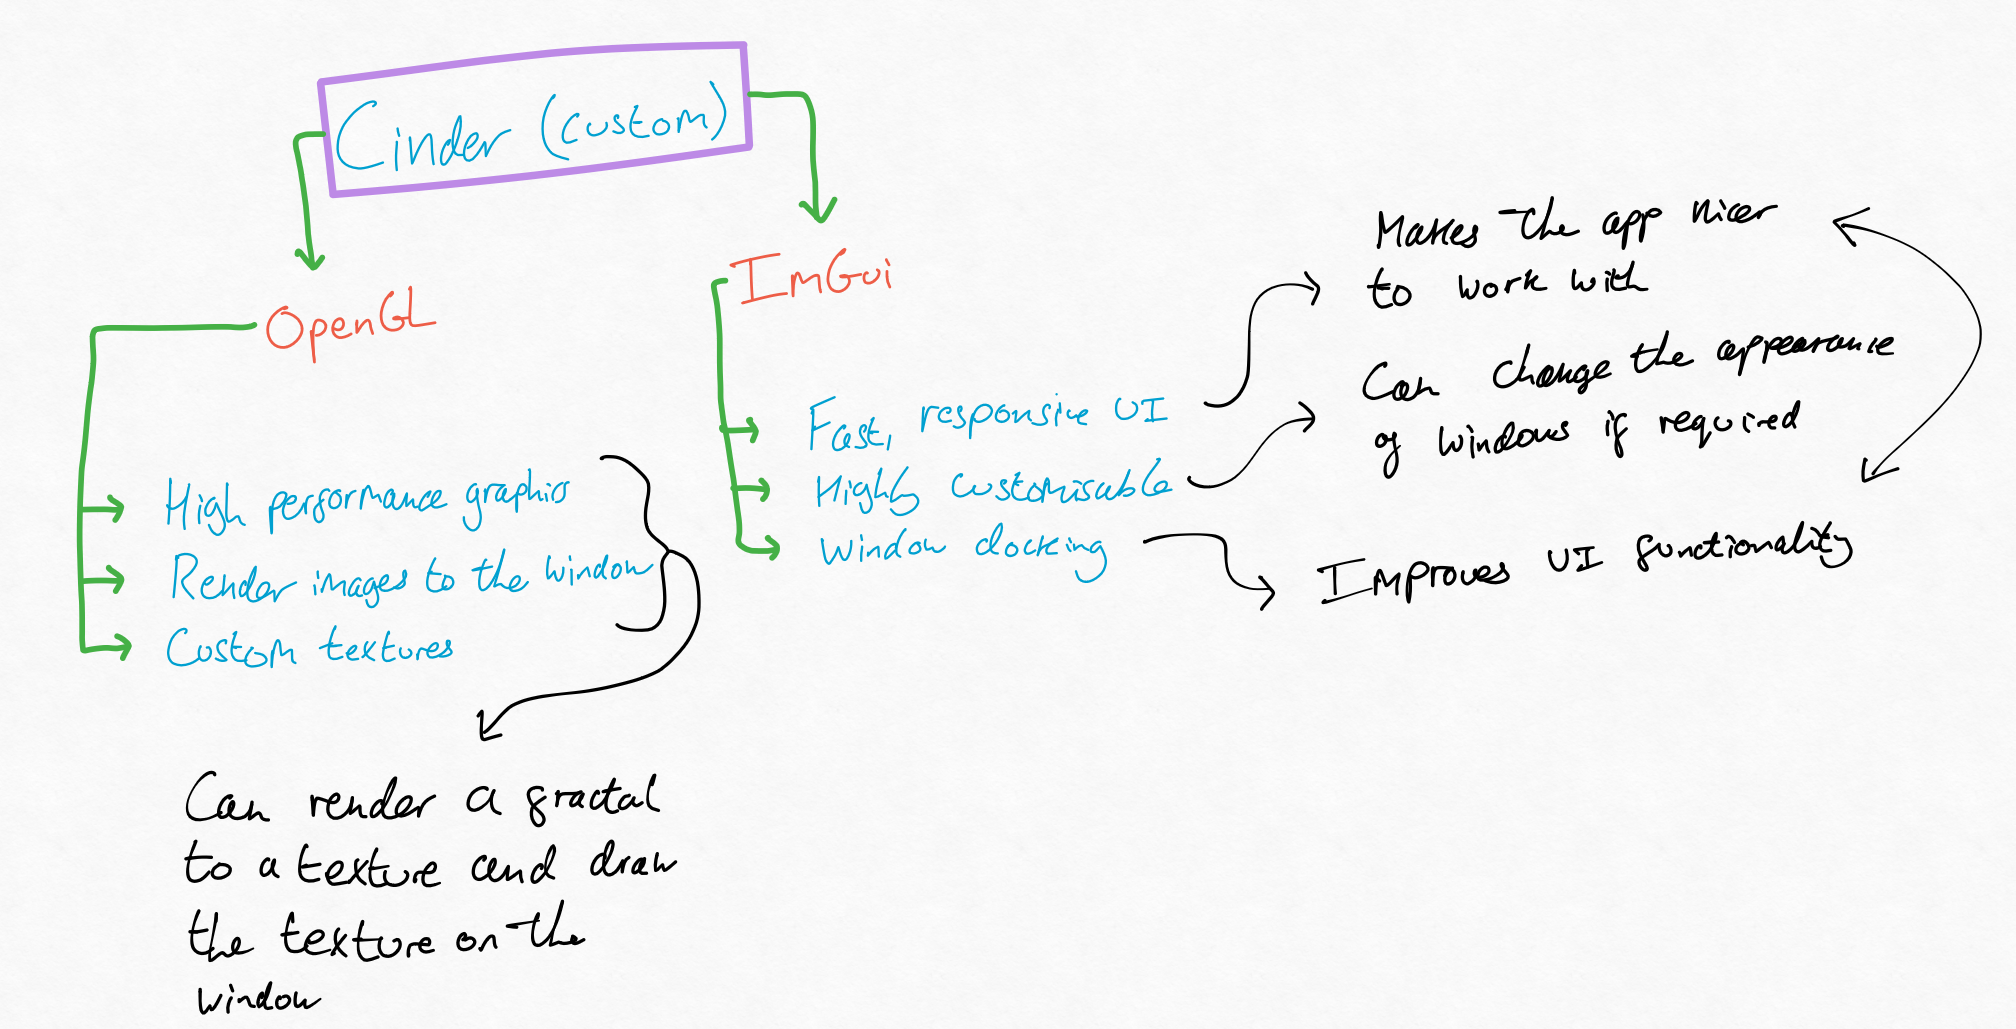
\includegraphics[width=\textwidth]{CinderLibraries.png}
\end{figure*}
\FloatBarrier

\FloatBarrier
\begin{figure*}[htp]
    \centering
    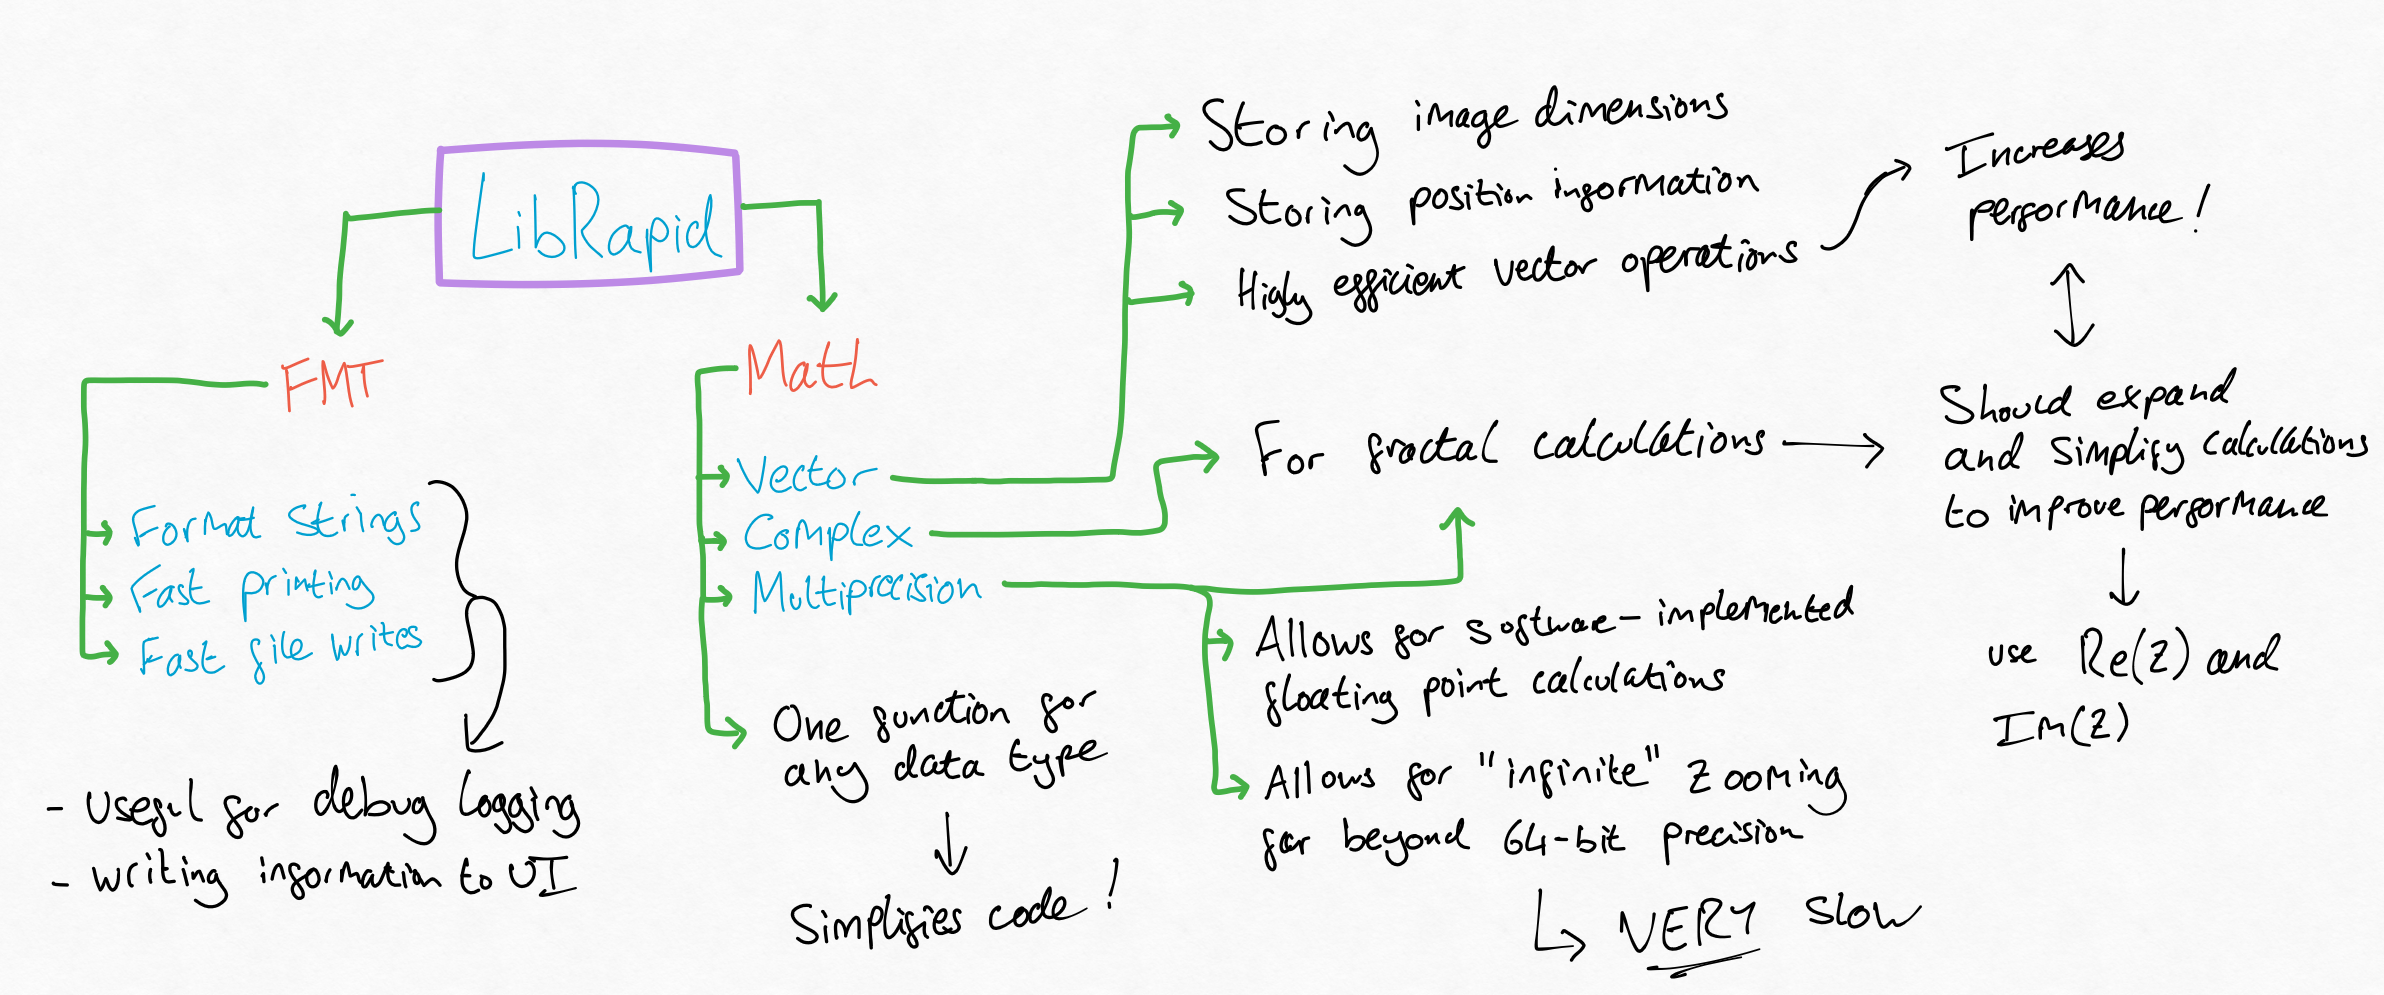
\includegraphics[width=\textwidth]{LibRapidLibraries.png}
\end{figure*}
\FloatBarrier

\subsection{The Debug Logger}

Since the program is written in \CPP and is a GUI application instead of a console application, there will not be a usable standard output to which debug information can be printed. To circumvent this issue, I will use a debug logger instance to write information to a file.

\FloatBarrier
\begin{figure*}[htp]
    \centering
    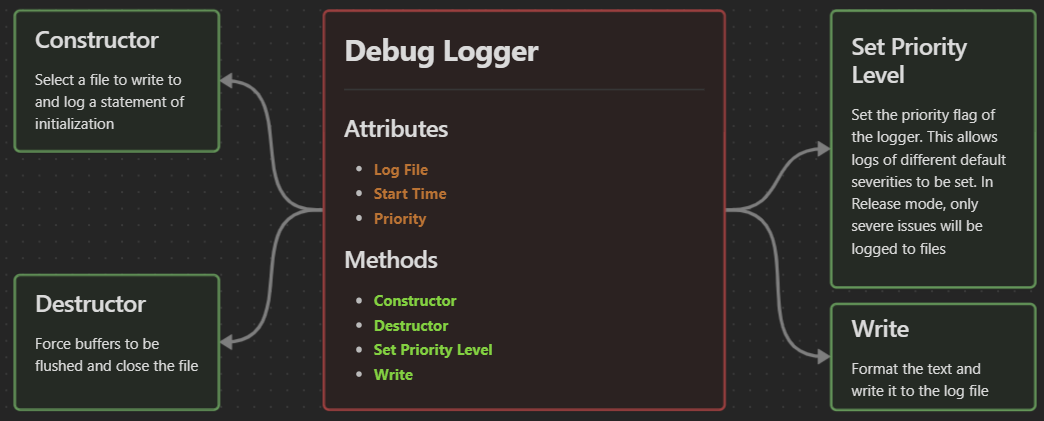
\includegraphics[width=\textwidth]{ClassDebugLogger.png}
\end{figure*}
\FloatBarrier

The logger's constructor will take a file path relative to the executable and attempt to open the specified file. If the document does not exist, it will be created for the user. The destructor will ensure that all buffers are flushed, and the file is closed. Without these checks, the program may terminate without saving the changes to be written to the file, and the debug log might be incomplete or corrupt. The logger will also have a priority level, optimising logging in release builds, as the user does not need all the information. For example, the logger could be configured to write only errors to the file in release mode. Finally, the logger has a function which enables the user to send data to be written to the file. New lines should be formatted appropriately, and logs should be timestamped. In addition to these functions, I will create a macro that captures the log statement's line number and filename, making tracebacks easier and faster during development.

\subsection{Colour Palettes}

A simple class containing a list of colours and a few helper methods is helpful for storing the colours and gradients used by the fractal rendering process. This class simplifies the act of colour palette generation and usage throughout the software, reducing bugs and improving the rate of development.

\FloatBarrier
\begin{figure*}[htp]
    \centering
    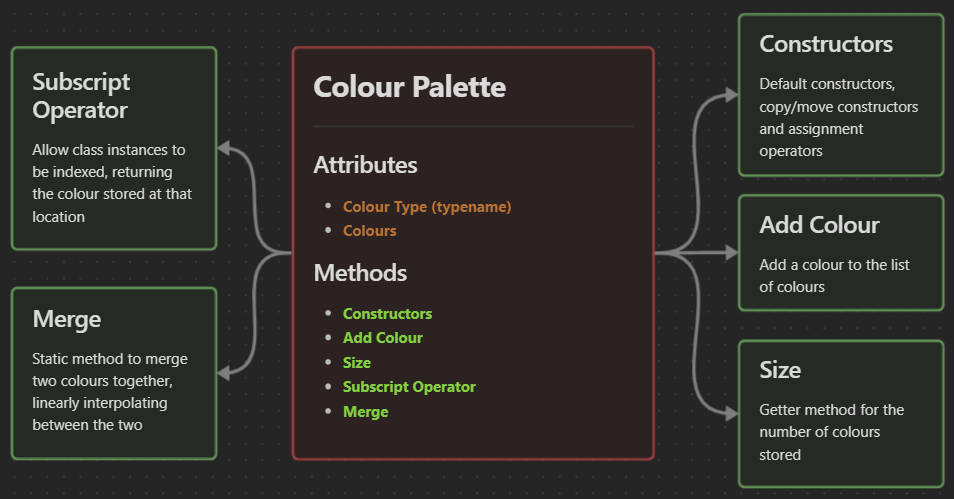
\includegraphics[width=\textwidth]{ClassColourPalette.png}
\end{figure*}
\FloatBarrier

The colour merging function is a very simple static method of the class, which linearly interpolates between the colour's red, green and blue components.

\begin{equation}
    \left\{ \phantom{\frac{a}{b}} t \times (R-r) + r, \quad t \times (G-g) + g, \quad t \times (B-b) + b \phantom{\frac{a}{b}} \right\}
\end{equation}

Where $t$ is the interpolation factor and $0 \le t \le 1$.

\subsection{The Fractal Class}

To support multiple fractal equations at runtime, each fractal will be implemented as a class inheriting from a main parent type. This is the fractal data type. It defines the functions required to iterate the fractal's equation from a given starting value, the logic to generate a colour from a starting point, an endpoint, and the number of iterations required to get there.

\FloatBarrier
\begin{figure*}[htp]
    \centering
    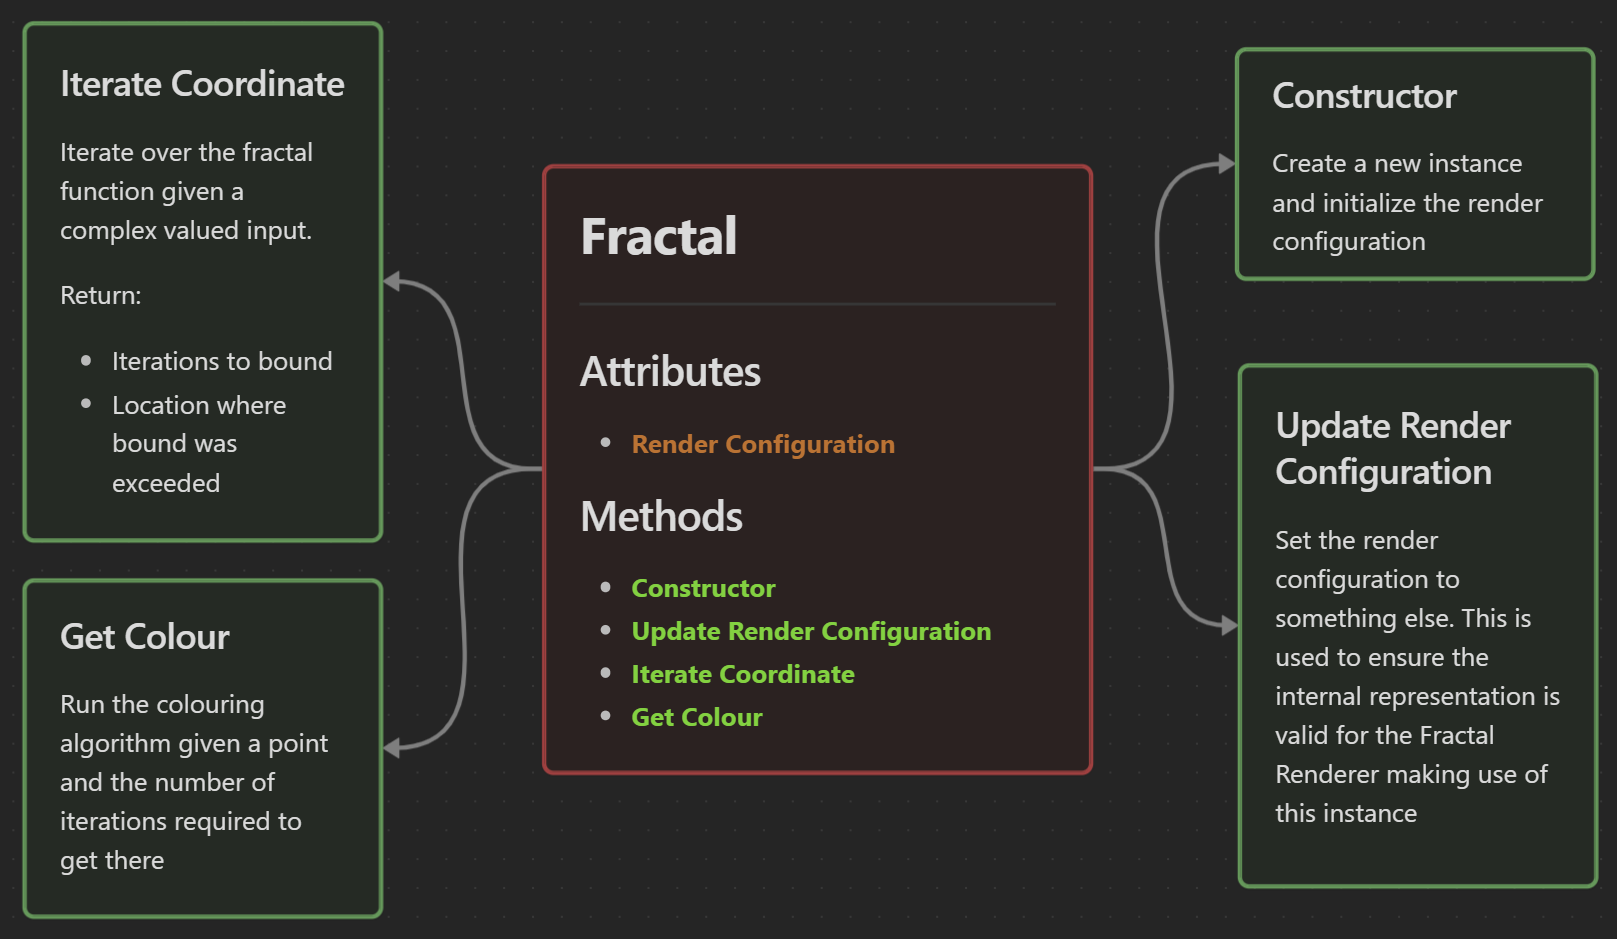
\includegraphics[width=\textwidth]{ClassFractal.png}
\end{figure*}
\FloatBarrier

\vspace{0.5cm}
\noindent
For example, the code below shows the definition of the Mandelbrot fractal class.

\begin{lstlisting}[language=c++]
#pragma once

#include <fractal/genericFractal.hpp>

namespace frac {
	class Mandelbrot : public Fractal {
	public:
		/// Constructor taking a RenderConfig object
		/// \param config RenderConfig object
		explicit Mandelbrot(const RenderConfig &config);
		Mandelbrot(const Mandelbrot &)			  = delete;
		Mandelbrot(Mandelbrot &&)				  = delete;
		Mandelbrot &operator=(const Mandelbrot &) = delete;
		Mandelbrot &operator=(Mandelbrot &&)	  = delete;

		~Mandelbrot() override = default;

		LIBRAPID_NODISCARD std::pair<int64_t, lrc::Complex<LowPrecision>>
		iterCoordLow(const lrc::Complex<LowPrecision> &coord) const override;

		LIBRAPID_NODISCARD std::pair<int64_t, lrc::Complex<HighPrecision>>
		iterCoordHigh(const lrc::Complex<HighPrecision> &coord) const override;
	};
} // namespace frac
\end{lstlisting}

\subsubsection{Render Box States}

An enum of valid states is required to keep track of each render box's current state. This is drawn to the main window on top of the fractal as it renders, providing the user with information about which areas are rendered, which are actively rendering and which areas are yet to be processed.

\begin{lstlisting}[language=c++]
/// Represents the state of a render box
enum class RenderBoxState {
    None,	   // Not yet assigned a state
    Queued,	   // Queued to be rendered
    Rendering, // Currently being rendered
    Rendered   // Rendered and ready to be written to the image
};
\end{lstlisting}

\subsubsection{Render Boxes}

The position information required to render a small area of the main fractal is contained within a \codeword{RenderBox} struct. These can be passed to a function inside the \codeword{FractalRenderer} class to be processed. 

\begin{lstlisting}[language=c++]
/// Stores the pixel-space coordinates of a region to render
struct RenderBox {
    lrc::Vec2i topLeft;
    lrc::Vec2i dimensions;
    RenderBoxState state = RenderBoxState::None;
    double renderTime	 = 0;
};
\end{lstlisting}

\subsubsection{Render Box Statistics}

To calculate the remaining time of the render and the fastest and slowest render box times, the program needs to know precisely how long each box took to render. To improve efficiency, a separate struct is created to store this data.

\begin{lstlisting}[language=c++]
struct RenderBoxTimeStats {
	double min	  = 0;
	double max	  = 0;
	double average = 0;
	double remainingTime = 0;
};
\end{lstlisting}

\subsubsection{Render Configurations}

Arguably the most important helper class, the \codeword{RenderConfig} struct contains all the information required for a \codeword{FractalRenderer} instance to render an image. The information in this struct can also be saved to a JSON file and shared, allowing people to send specific configurations between users easily.

\begin{lstlisting}[language=c++]
struct RenderConfig {
	int64_t numThreads; // Number of threads to render on (max)
	int64_t maxIters;	// Largest number of iterations to allow
	int64_t precision;	// Precision (in bits) of floating point types used for arithmetic
	LowPrecision bail;	// Bailout value
	int64_t antiAlias;	// Anti-aliasing factor -- 1 = no anti-aliasing
	lrc::Vec2i imageSize; // Size of the image to render
	lrc::Vec2i boxSize;	  // Size of sub-regions to render (see RenderBox)
	lrc::Vec<HighPrecision, 2> fracTopLeft;		 // The fractal-space center of the image
	lrc::Vec<HighPrecision, 2> fracSize;		 // The width and height of the fractal space
	lrc::Vec<HighPrecision, 2> originalFracSize; // Original size for zoom factor calculation
	ColorPalette palette; // The palette to use for rendering the fractal
};
\end{lstlisting}

\subsection{The Fractal Renderer Class}

While it is essential to have a method of calculating the colour of a given point on the fractal (from the fractal class), it doesn't support rendering an entire image. This is the role of the fractal renderer class.

\FloatBarrier
\begin{figure*}[htp]
    \centering
    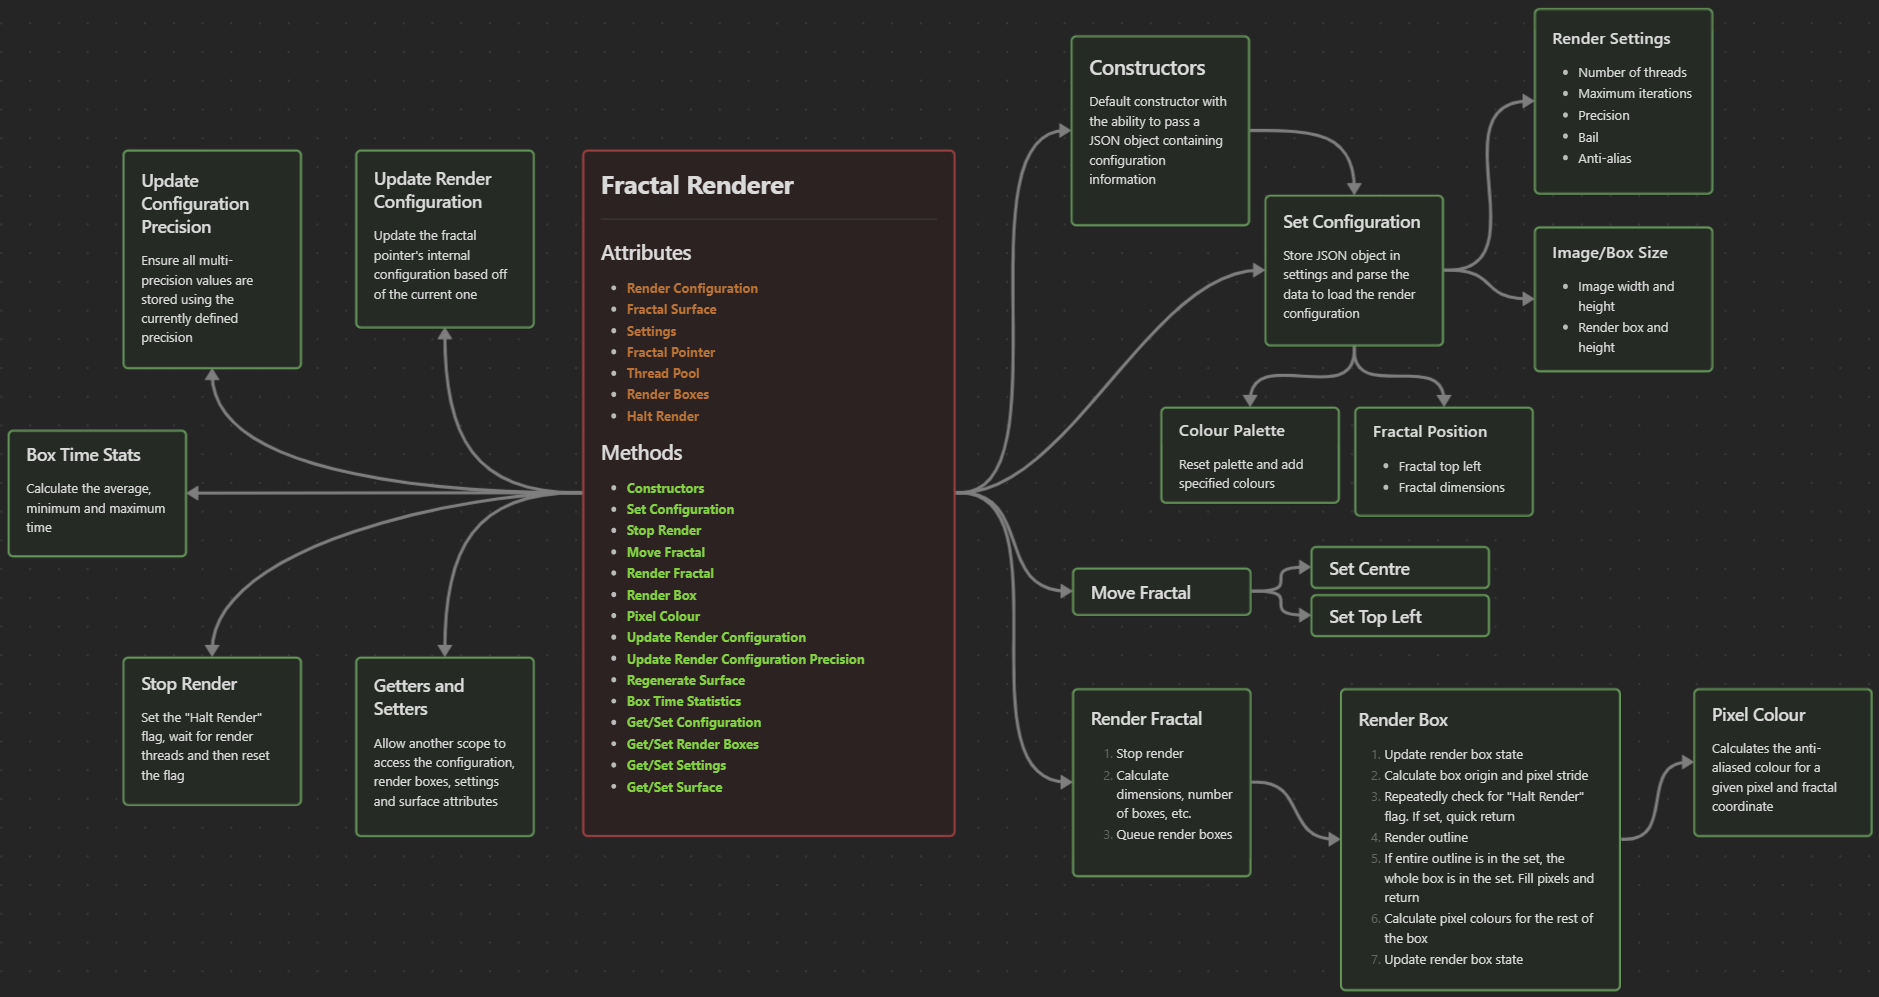
\includegraphics[width=\textwidth]{ClassFractalRenderer.png}
\end{figure*}
\FloatBarrier

This class implements many functions at various levels of abstraction, allowing performance-critical sections of the code to be run with efficient, parallelised algorithms. At the same time, the high-level interfaces are easy to interact with and use.

\subsubsection{Configuration, Getters, Setters and Statistics}

\FloatBarrier
\begin{figure*}[htp]
    \centering
    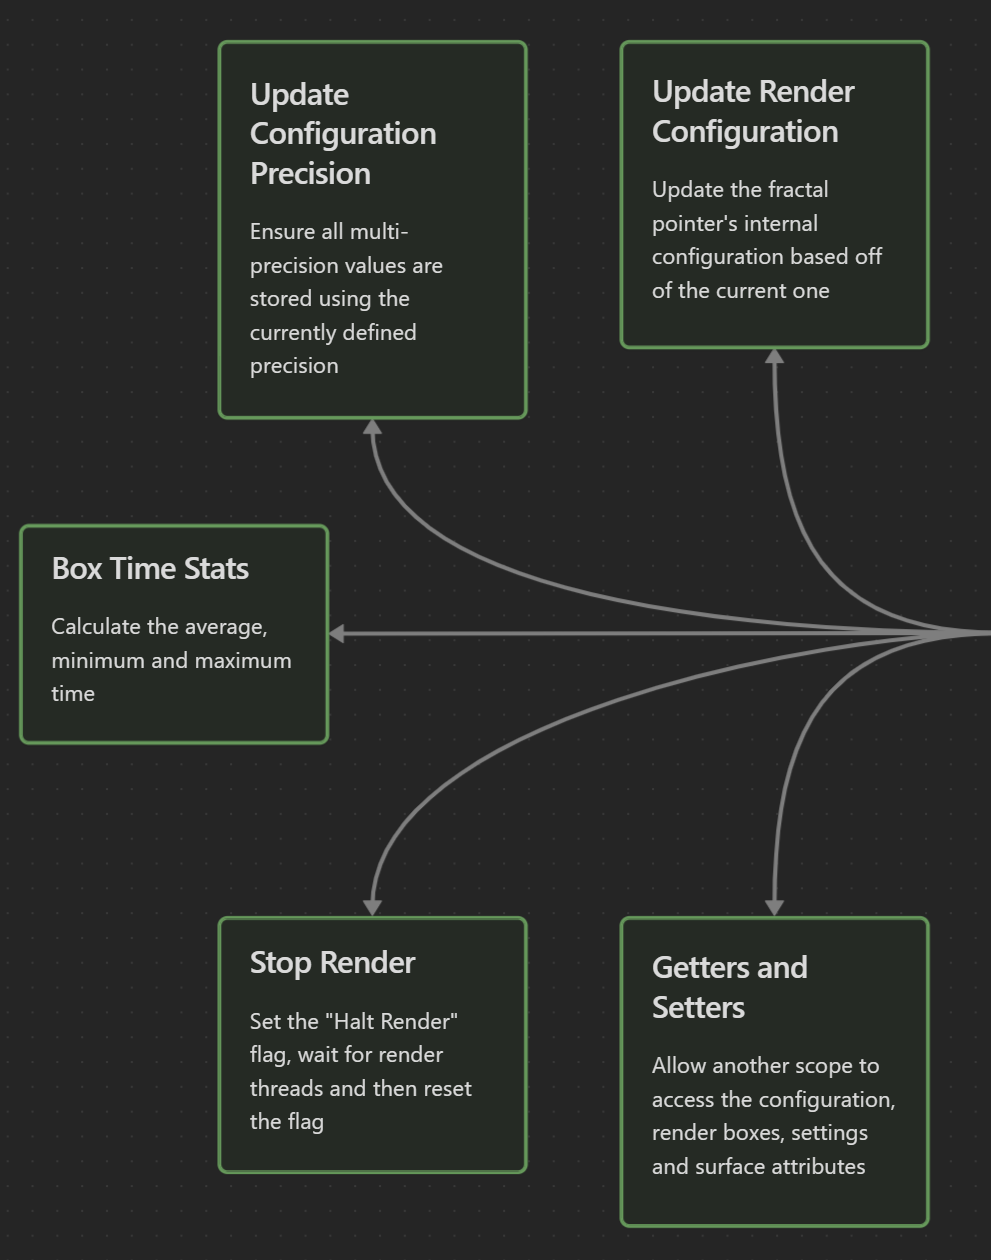
\includegraphics[width=\textwidth]{ClassFractalRendererLeftSide.png}
\end{figure*}
\FloatBarrier

These functions operate at a high level, allowing basic access to the information stored by the class. While simple, they are essential for the main program to function correctly, as there would be no way of accessing the rendered image, for example.

\subsubsection{Constructors and Configurations}

\FloatBarrier
\begin{figure*}[htp]
    \centering
    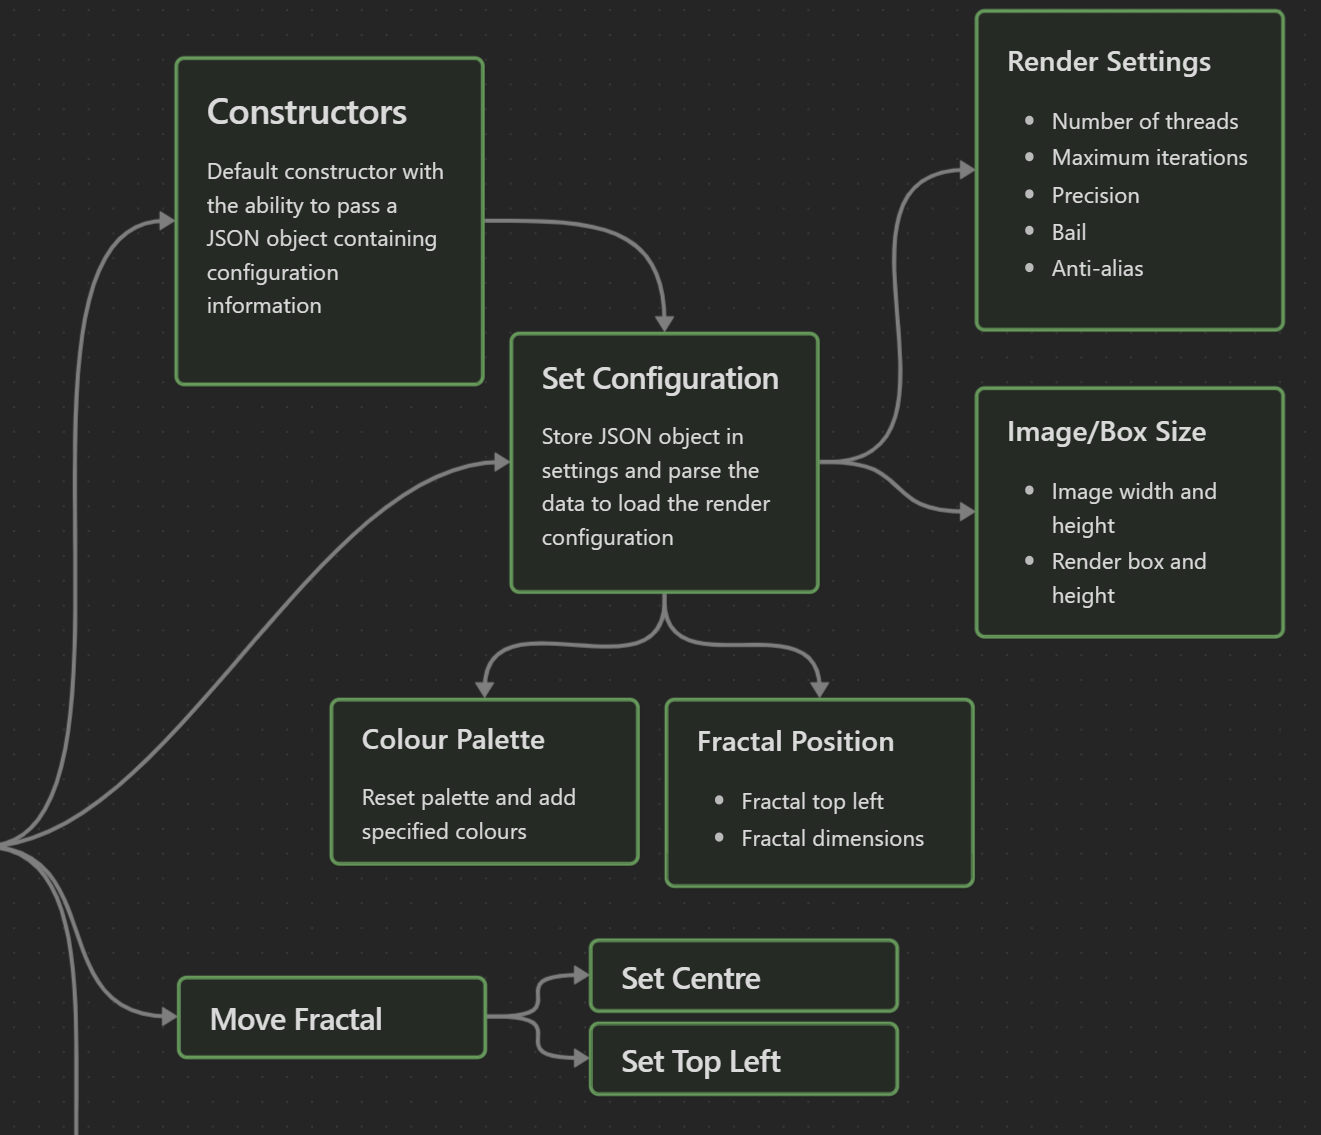
\includegraphics[width=\textwidth]{ClassFractalRendererTopRightSide.png}
\end{figure*}
\FloatBarrier

To render a fractal, much information is required about the dimensions of the image, the dimensions of the fractal, the origin in the complex plane, and more.

The fractal renderer class can parse a JSON object and load its configuration. By storing some data as a string instead of a number, it is possible to save and load high-precision numbers as well -- this could be used to enable fractal locations with extremely high zoom factors to be saved and shared easily.

\vspace{0.5cm}
\noindent
The JSON snippet below shows a highly simplified version of the default configuration used within the software (for a full version, see the code-listing at the end of the document).

% Using language=python to change syntax highlighting
\begin{lstlisting}[language=python]
{
	"renderConfig": {
		"numThreads": 8,
		"maxIters": 500,
		"precision": 64,
		"bail": 65536,
		"antiAlias": 2,
		"imageSize": {
			"width": 800,
			"height": 700
		},
		"colorPalette": [
			{
				"red": 0.5568628,
				"green": 0.23137255,
				"blue": 0.27450982,
				"alpha": 1.0
			},
			{
				"red": 0.88235295,
				"green": 0.8666667,
				"blue": 0.56078434,
				"alpha": 1.0
			}
		]
	}
}
\end{lstlisting}

A vast number of configuration options can be configured in the file, including the threading options, render quality settings and even the size of the boxes to render in parallel.

The \codeword{loadConfiguration} method also enables the configuration to be changed or re-parsed at runtime, allowing quick and easy updates to the fractal settings.

\subsubsection{Rendering Algorithms}

\FloatBarrier
\begin{figure*}[htp]
    \centering
    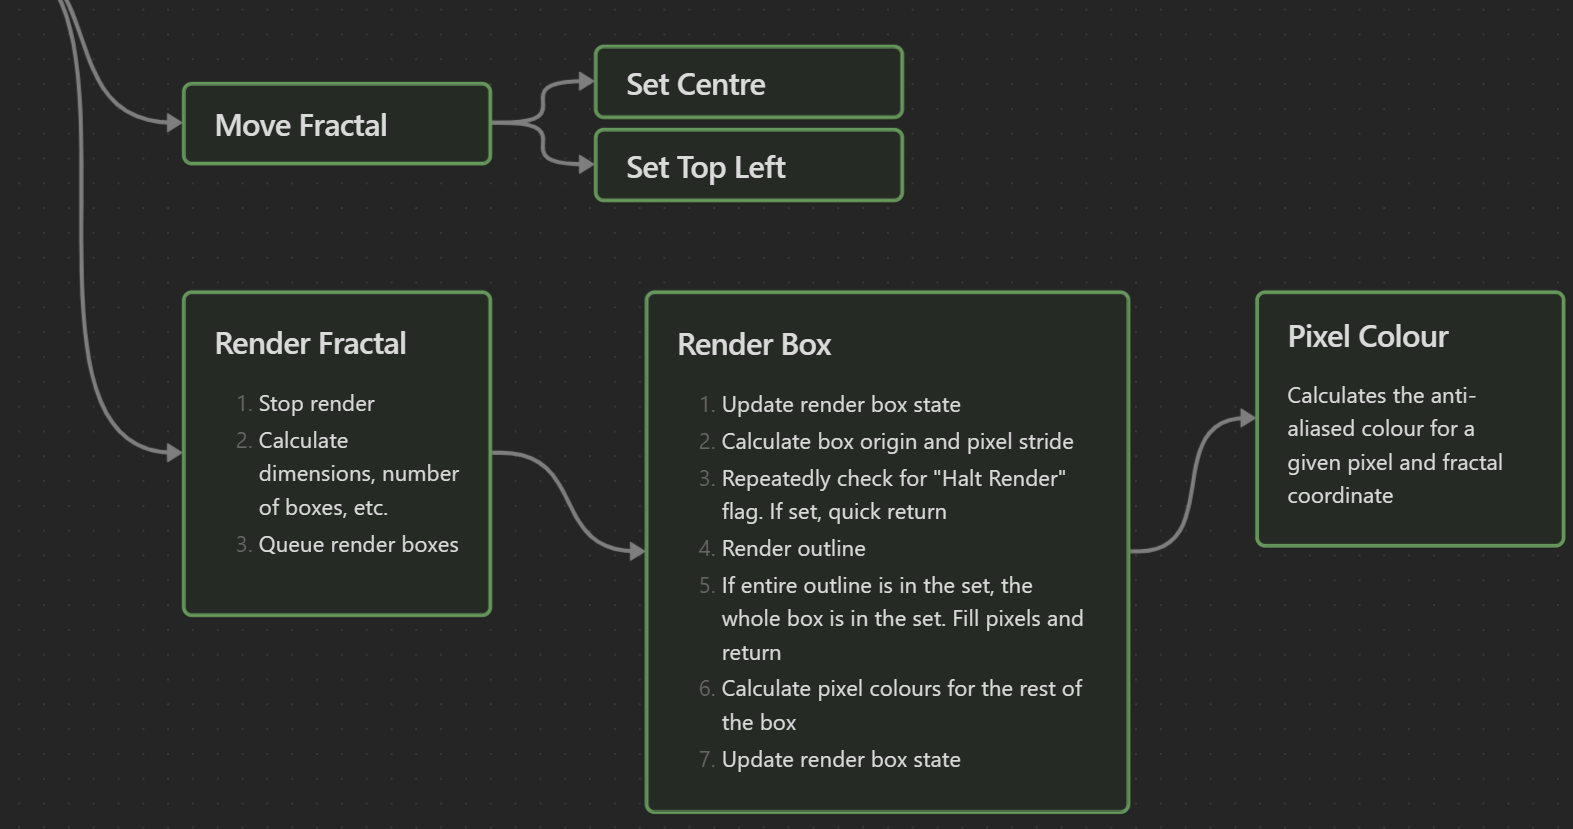
\includegraphics[width=\textwidth]{ClassFractalRendererBottomRightSide.png}
\end{figure*}
\FloatBarrier

The fractal renderer is responsible for creating an image buffer and setting the colour of each pixel in that image to represent the fractal at that location. Doing this efficiently is difficult, so the process is split into many small functions, providing fine-grained control over the algorithm.

Upon requesting the renderer to re-render the image, any existing render threads are halted, dependent image settings are recalculated, and the render-box queue is cleared.

Next, the render boxes are recalculated and pushed back to the render queue. Each box is dequeued by a thread in a thread pool and runs in parallel.

To optimise the rendering of each box, we can use the fact that if an outline can be drawn where every point is in the set, every point contained within that outline must also be within the set. Outlining each box before calculating the inner area makes it possible to check whether all points were in the set. If they were, we can quickly fill the rest of the box without calculating the colour of each pixel.

To calculate the colour of each pixel, we first call the \codeword{iterCoord} method of the fractal pointer stored to get the number of iterations required to exceed the bailout value (if it is exceeded at all), as well as the first point at which this occurs. This information is then passed to the fractal's colouring algorithm to generate a colour for the pixel. If anti-aliasing is enabled, this process is repeated for multiple points within the pixel, and the resulting colours are averaged. Anti-aliasing produces smoother images that appear to be higher resolution, allowing for faster render times with high-quality results.

The fractal renderer class also implements routines to change the fractal-space coordinates to render. This is used to move the fractal when zooming in or out. For different use cases, there are methods to set the top left coordinate or the image's centre.

\subsection{The Main Window}

\FloatBarrier
\begin{figure*}[htp]
    \centering
    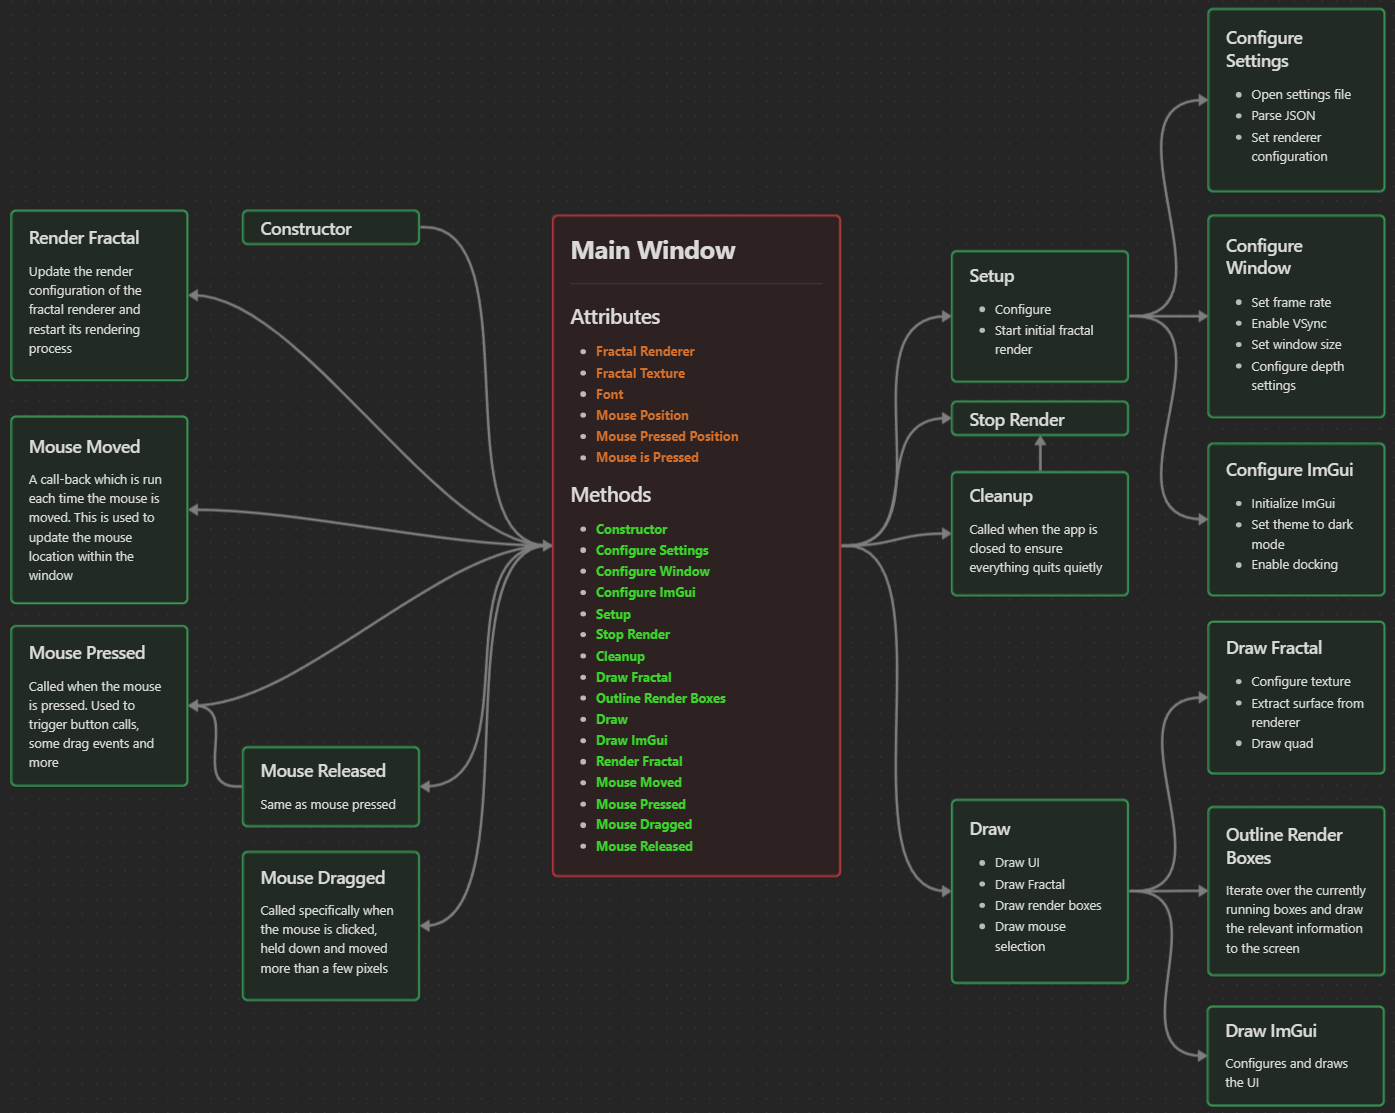
\includegraphics[width=\textwidth]{ClassMainWindow.png}
\end{figure*}
\FloatBarrier

This class is responsible for creating, managing and drawing information to the window and controlling all the other classes mentioned previously.

\vspace{0.5cm}
\noindent
When the window is created by \textit{Cinder}, the \codeword{setup} routine is called, initializing the window's attributes. First, the settings JSON file is loaded, parsed and passed to the fractal renderer member. Next, the window itself is constructed and configured, including the framerate, enabling or disabling vertical syncing (V-Sync), the window size and OpenGL depth buffer settings. Finally, \textit{ImGui} is configured.

The \codeword{MainWindow} class is also responsible for drawing to the window. After setting the background colour, the \textit{ImGui} windows are created and drawn. This produces most of the UI, but some extra parts must be drawn in later. Next, the fractal itself is drawn to the screen. An image texture is created and assigned the fractal image buffer, and a rectangle is drawn with the aforementioned texture. The rest of the UI is now drawn, including the render-box status indicators and the mouse selection.

When the application is requested to close, the \codeword{cleanup} routine is called. This signals any existing render threads to halt, ensures all members are correctly destructed and then destroys the window.

The window also has a variety of callback functions which are called when specific triggers occur. For example, functions are called every time the mouse is moved, dragged or pressed.

\subsection{Additional Features}

The features outlined previously comprise the vast majority of the program, but some additional features must also be designed and implemented. These are often the less critical features, though they still impact the user's interaction with the program.  

\subsubsection{Movement History}

While we often take the ``undo'' and ``redo'' buttons for granted, they give us a powerful means of reverting unwanted changes. Furthermore, they allow the user to see what adjustments have been made to the fractal between movements, supporting verbal descriptions of how to arrive at fascinating points within the fractal.

Using a linked list, where each node stores a \codeword{RenderConfig} object and a \codeword{Surface}, it is possible to implement a move history into the program. Whenever the user requests to change a setting or move the origin of the fractal, the current surface and render configuration are appended to the history before the changes are applied.

\begin{center}
	\begin{tikzpicture}
		\node (classDef) [boxNode] {
			$
			\begin{aligned}
				&\textbf{HistoryNode} \\ \\
				&\codeword{HistoryNode *m_next} \\
				&\codeword{HistoryNode *m_prev} \\
			\end{aligned}
			$
		};
		\node (appendFn) [boxNode, below of = classDef, node distance = 100pt] {
			$
			\begin{gathered}
				\codeword{append(HistoryNode *node)}
			\end{gathered}
			$
		};
		\node (ifStatement) [conditionNode, below of = appendFn, node distance = 100pt] {
			$
			\begin{gathered}
				\codeword{m_next} \text{ is } \codeword{NULL}?
			\end{gathered}
			$
		};
	
		\node (ifPoint) [square, right of = ifStatement, node distance = 180pt] {no};
		
		\node (recurse) [boxNode, right of = appendFn, node distance = 180 pt] {
			$
			\begin{gathered}
				\text{Call } \codeword{append} \text{ on } \codeword{m_next}
			\end{gathered}
			$
		};
		
		\node (assignStatement) [boxNode, below of = ifStatement, node distance = 100pt] {
			$
			\begin{aligned}
				& \text{Assign } \codeword{node} \text{ to } \codeword{m_next}
			\end{aligned}
			$
		};
		
		\draw [arrow] (classDef) -- (appendFn);
		\draw [arrow] (appendFn) -- (ifStatement);
		\draw (ifStatement) -- (ifPoint);
		\draw [arrow] (ifPoint) -- (recurse);
		\draw [arrow] (recurse) -- (appendFn);
		\draw [arrow] (ifStatement) -- (assignStatement);
	\end{tikzpicture}
\end{center}

\subsubsection{Improved Selection Area}
